
%\documentstyle[epsf,twocolumn]{jarticle}       %LaTeX2e仕様
\documentclass[twocolumn]{jarticle}     %pLaTeX2e仕様(platex.exeの場合)
% \documentclass[onecolumn]{ujarticle}   %pLaTeX2e仕様(uplatex.exeの場合)
%%%%%%%%%%%%%%%%%%%%%%%%%%%%%%%%%%%%%%%%%%%%%%%%%%%%%%%%%%%%%%
%%
%%  基本バージョン
%%
%%%%%%%%%%%%%%%%%%%%%%%%%%%%%%%%%%%%%%%%%%%%%%%%%%%%%%%%%%%%%%%%
\setlength{\topmargin}{-45pt}
%\setlength{\oddsidemargin}{0cm}
\setlength{\oddsidemargin}{-7.5mm}
%\setlength{\evensidemargin}{0cm}
\setlength{\textheight}{24.1cm}
%setlength{\textheight}{25cm}
\setlength{\textwidth}{17.4cm}
%\setlength{\textwidth}{172mm}
\setlength{\columnsep}{11mm}

%\kanjiskip=.07zw plus.5pt minus.5pt


% 【節が変わるごとに (1.1)(1.2) … (2.1)(2.2) と数式番号をつけるとき】
%\makeatletter
%\renewcommand{\theequation}{%
%\thesection.\arabic{equation}} %\@addtoreset{equation}{section}
%\makeatother

%\renewcommand{\arraystretch}{0.95} 行間の設定
%%%%%%%%%%%%%%%%%%%%%%%%%%%%%%%%%%%%%%%%%%%%%%%%%%%%%%%%
%\usepackage{graphicx}   %pLaTeX2e仕様(\documentstyle ->\documentclass)
\usepackage[dvipdfmx]{graphicx}
\usepackage{subcaption}
\usepackage{multirow}
\usepackage{amsmath}
\usepackage{url}
\usepackage{ulem}
\usepackage{algorithm}
\usepackage{algorithmic}
\usepackage{listings} %,jlisting} %日本語のコメントアウトをする場合jlistingが必要
%ここからソースコードの表示に関する設定
\lstset{
  basicstyle={\ttfamily},
  identifierstyle={\small},
  commentstyle={\smallitshape},
  keywordstyle={\small\bfseries},
  ndkeywordstyle={\small},
  stringstyle={\small\ttfamily},
  frame={tb},
  breaklines=true,
  columns=[l]{fullflexible},
  numbers=left,
  xrightmargin=0zw,
  xleftmargin=3zw,
  numberstyle={\scriptsize},
  stepnumber=1,
  numbersep=1zw,
  lineskip=-0.5ex
}
\newcommand{\argmax}{\mathop{\rm arg~max}\limits}
\newcommand{\argmin}{\mathop{\rm arg~min}\limits}

%%%%%%%%%%%%%%%%%%%%%%%%%%%%%%%%%%%%%%%%%%%%%%%%%%%%%%%%
\begin{document}

	%bibtex用の設定
	%\bibliographystyle{ujarticle}

	\twocolumn[
		\noindent
		\hspace{1em}
		2021 年 6 月 28 日
		発表資料
		\hfill
		M1 杉山 竜弥
		\vspace{2mm}

		\hrule
		\begin{center}
			{\Large \bf 仮タイトル}
		\end{center}
		\hrule
		\vspace{9mm}
	]

\section{はじめに}
GPT-2\cite{radford2019language}を実行した.
GPTとその前提のtransformer\cite{DBLP:journals/corr/VaswaniSPUJGKP17}について調査した.

\section{要素技術}
\subsection{Transformer}
Transformer\cite{DBLP:journals/corr/VaswaniSPUJGKP17} は再帰的ニューラルネットワーク (Recurrent Neural Network: RNN)\cite{mikolov2010recurrent} を使わずに, Self-Attention を使って並列計算を可能にするモデルである.

RNN は時系列に沿って順番に計算する構造であるため並列計算ができず,
GPU などを使っても計算時間が長いという欠点がある.
GPU の性能を十分に活用し, 計算速度を向上させるため, RNN を使用しないことが必要となる.

% Self-Attentionとは、attentionの実践のところで紹介しましたが、もともとの論文にあった 翻訳語の単語から翻訳前の単語に注意を向けるattentionではなく、自分自身のどこが重要かに注意を向ける.
Self-Attentionは, シーケンス内の単語間の関係性に注目する.

Positional Encoding



\begin{figure}[tb]
  \begin{center}
    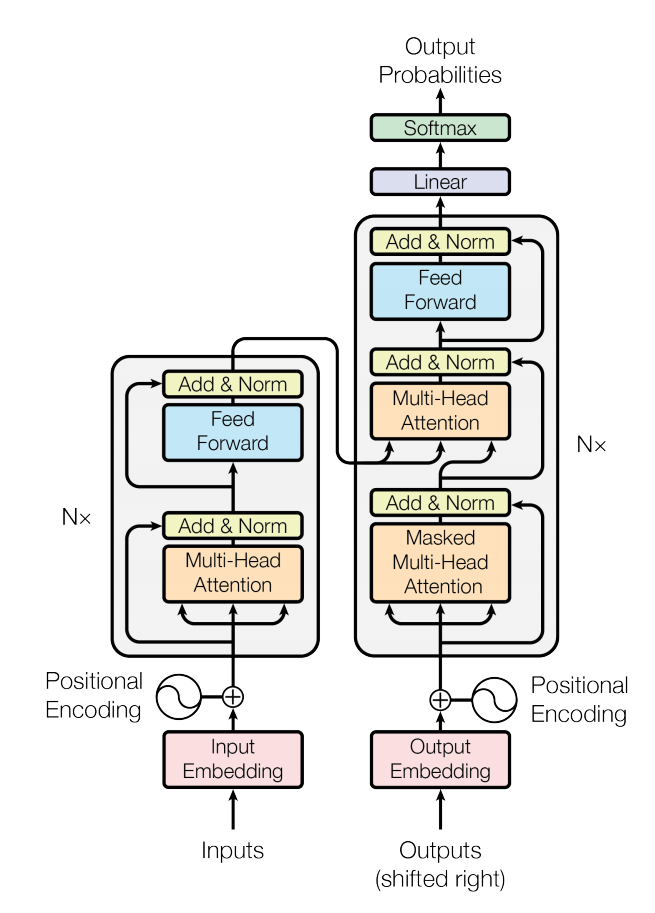
\includegraphics[clip,width=75mm]{Transformer.png}
    \caption{Transformer}
    \label{fig:trans}
  \end{center}
\end{figure}



\subsection{GPT-2}
Generative Pretrained Transformer 2 (GPT-2)\cite{radford2019language} は
% 特定のタスクに特化した教師あり学習は行わず、より大きな言語コーパスを使って、より大きなモデルの言語モデルを事前学習させることにより、zero-shot、もしくはfew-shotのセッティングでも精度が出るような汎用的なモデルを目指しています。
% zero-shot もしくは few-shot のデータでも精度が出るような汎用的なモデルである.
特定のタスクに特化した数万の教師ありデータでファインチューニングが必要だった GPT, BERT をはじめとしたモデルと異なり,
大規模な言語コーパスで様々なタスクを学習する汎用的なモデルとして設計された.

 % variable length sequences of symbols
任意の長さの文章をシンボルにしたシーケンスを $(s_1, s_2, ..., s_n)$ とする.
同時確率は条件付確率の積に分解される.
\begin{equation}
p(x) = \prod^n_{i=1} p(s_n|s_1, ... , s_{n-1})
\end{equation}
この条件付確率は, Transformer\cite{DBLP:journals/corr/VaswaniSPUJGKP17}によって効率的に計算できる.

GPT-2では, $p(\mathrm{output}|\mathrm{input})$ を一般化して,
$p(\mathrm{output}| \mathrm{input}, \mathrm{task})$と表しタスクの種類も学習することで, 特定の問題のためのファインチューニングなしで, 1つのモデルでも問題を解けるようにしている.


% Fine-tuning
% 次に言語モデルのファインチューニングと分類器のファインチューニングを行います。
% ULMFiTではこれらを順番に行っていましたが、OpenAI GPTでは同時に行うようです。
%
% 両方ともラベル付きデータを使って行います。
% ラベル付きデータの入力単語をx1,⋯,xmとすると、ラベルyの予測は最後のtransformer blockの最後の時点の出力hmlのベクトルを使ってsoftmaxレイヤーにより求めます。
%
% P(y|x1,⋯,xm)=softmax(hmlWy)
% そして、ラベル付きデータをCとすると、対数尤度
%
% L2(C)=∑(x,y)logP(y|x1,⋯,xm)
% が最大になるようにパラメータを調整します。
% さらに、単純にL2を最大化させるのではなく、同時に言語モデルのファインチューニングを行います。
% その尤度をL3とすると、
%
% L3(C)=L2(C)+λ∗L1(C)
% を最大化するように、言語モデルと分類器のファインチューニングを同時に行います。
% L1(C)は ラベル付きコーパスを使った言語モデル(Pretrainingのところの式)の学習を意味しています。
% この目的関数をauxiliary objectiveと呼んでいます。


\begin{table}[tbh]
  \begin{center}
    \caption{GPT-2の解けるタスク}
    \begin{tabular}{|c|} \hline
      AutomaticSpeechRecognition \\ \hline
      Conversational \\ \hline
      FeatureExtraction \\ \hline
      FillMask \\ \hline
      ImageClassification \\ \hline
      QuestionAnswering \\ \hline
      Summarization \\ \hline
      TextClassification \\ \hline
      TextGeneration \\ \hline
      TokenClassification \\ \hline
      Translation \\ \hline
      ZeroShotClassification \\ \hline
      % Text2TextGeneration \\ \hline
      % TableQuestionAnswering \\ \hline
    \end{tabular}
    \label{tab:task}
  \end{center}
\end{table}

\subsection{Byte Pair Encoding}
Byte Pair Encoding (BPE) は高頻度の単語は単語全体を辞書に登録し、低頻度の単語は文字単位に分割する言語モデルにおける未知語処理手法である.

言語モデルは語彙サイズをハイパーパラメータとして設定するため, ニューラルモデルに扱われない未知語が存在する.
未知語処理として, $<unk>$ などの特殊トークンに置き換える方法と, 単語をより細かく分割しサブワードにすることで語彙を少なくする方法がある.

BPE は
データ圧縮手法を言語モデルに応用した.
文字単位に単語を分解し, 2 文字のペアの中で高頻度の要素を結合して 1 つのサブワードとする手順を繰り返すことで,
単語を接頭辞や接尾辞などの意味のある単位に分解できる.


% \begin{figure}[tb]
%   \begin{center}
%     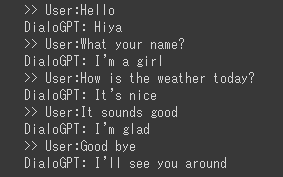
\includegraphics[clip,width=75mm]{ss.png}
%     \caption{対話例}
%     \label{fig:con}
%   \end{center}
% \end{figure}
%

% % \begin{table}[tb]
% %   \begin{center}
% %     \caption{GPT-2の解けるタスク}
% %     \begin{tabular}{|c|} \hline
% %       % AutomaticSpeechRecognition \\ \hline
% %       Conversational \\ \hline
% %       % FeatureExtraction \\ \hline
% %       % FillMask \\ \hline
% %       % ImageClassification \\ \hline
% %       QuestionAnswering \\ \hline
% %       Summarization \\ \hline
% %       TextClassification \\ \hline
% %       TextGeneration \\ \hline
% %       % TokenClassification \\ \hline
% %       Translation \\ \hline
% %       % ZeroShotClassification \\ \hline
% %       % Text2TextGeneration \\ \hline
% %       % TableQuestionAnswering \\ \hline
% %     \end{tabular}
% %     \label{tab:task}
% %   \end{center}
% % \end{table}

\section{実験}

\subsection{対話タスク}

図 \ref{fig:con} に対話例を示した.
英語の場合, 対話を自然に続けられることを確認した.

\begin{figure}[tb]
  \begin{center}
    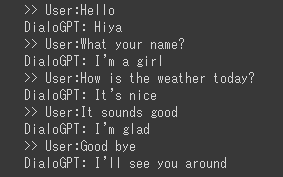
\includegraphics[clip,width=75mm]{ss.png}
    \caption{対話例}
    \label{fig:con}
  \end{center}
\end{figure}



% 参考文献リスト
\bibliographystyle{unsrt}
\bibliography{ref}
\end{document}
